\documentclass{jsarticle}
\usepackage[margin = .7in]{geometry}
\usepackage[dvipdfmx]{graphicx}
\usepackage{listings}
\usepackage{amsmath}
\usepackage{amsfonts}
\usepackage{bm}
\lstset{%
  language={python},
  basicstyle={\small},%
  identifierstyle={\small},%
  commentstyle={\small\itshape},%
  keywordstyle={\small\bfseries},%
  ndkeywordstyle={\small},%
  stringstyle={\small\ttfamily},
  frame={tb},
  breaklines=true,
  columns=[l]{fullflexible},%
  numbers=left,%
  xrightmargin=0zw,%
  xleftmargin=3zw,%
  numberstyle={\scriptsize},%
  stepnumber=1,
  numbersep=1zw,%
  lineskip=-0.5ex%
}

\begin{document}
\title{卒論テーマ候補 :満員電車}
\author{池上 慧}
\maketitle

\section{目的}
満員電車の緩和を目指す。このモデルでは各人が限定的であれprivate informationを申告することで社会的な損失を軽減できることが示唆される。最終的には、正直申告をさせるメカニズムに基づいて実際に乗車時間を事前に投票するアプリを用いた実証実験につなげたい。

\section{モデルの分析}
電車の候補が全部で$M$本とし、$j \in M$で各電車を指すとする。プレイヤーは$N$人で$i$をインデックスとする。プレイヤー$i$が電車$j$に乗車することの効用$(V_j^i)$は、その電車の発車時刻$(t_j)$に紐付いた$i$ごとに異なる価値$(u_j^i)$と、その電車に乗車するプレイヤーの数$(N_j)$に依存して決定する。ただし$\left\{u_j^i\right\}$は自身の持つ各電車への価値は自分で認識できるが、自分以外のプレイヤーが持つ各電車への価値は認識できないとする。ここでそれぞれの効用への寄与は分離できるとして、
\begin{align*}
	V_j^i = u_j^i + g(N_j)
\end{align*}
で書くことができるとする。

しかし、実際に乗車する電車を決定する際には、実現する乗車人数$N_j$に基づいて意思決定することはできない。なぜならまだその人数は実現していないからである。そのため、$N_j$についての期待値に基づいて意思決定を下すことになる。ここで、プレイヤー同士にも、経済学者にも観測できない撹乱項$\epsilon_j^i$が電車とプレイヤーについて独立に第1種極値分布にしたがうと仮定し、$additive$に効用に影響するとする。すなわち、
\begin{align*}
	h_j^i = V_j^i + \epsilon_j^i = u_j^i + g(N_j) + \epsilon_j^i
\end{align*}
でプレイヤー$i$の持つ電車$j$の効用をかけるとし、$N_j$について期待値をとった形で
\begin{align*}
	{h_j^i}^* = {V_j^i}^* + \epsilon_j^i = u_j^i + E[g(N_j)] + \epsilon_j^i
\end{align*}
と書くとする。
この時、$g(N_k) = \alpha N_k$として特定化すると、プレイヤー$i$が電車$j$を選ぶ確率は以下のようにかける。
\begin{align*}
	p_j^i = Pr(\text{i chooses j}) = P({h_j^i}^* \geq {h_{j^{'}}^i}^*\ \text{for all}\ j \in M) = \frac{\exp({V_j^i}^*)}{\sum_k \exp({V_k^i}^*)} = \frac{\exp(u_j^i + \alpha E[N_j])}{\sum_k \exp(u_k^i + \alpha E[N_k])}
\end{align*}

以下、簡単のためにプレイヤーの数と電車の数を共に$2$としてモデルを分析する。$p_2^1 = 1 - p_1^1$と$p_2^2 = 1 - p_1^2$より、先の結果を書き下すと、
\begin{align*}
	\begin{cases}p_1^1 &= \frac{1}{1 + \exp(u_2^1 - u_1^1 + 2\alpha(1 - p_1^1 - p_1^2))} \\[10pt]
	p_1^2 &= \frac{1}{1 + \exp(u_2^2 - u_1^2 + s\alpha(1 -p_1^1 -p_1^2))}
	\end{cases}
\end{align*}
のようにかける。

解釈として、$\left\{ p_j^i\right\}$は確率そのものではなく、新たに得られた各電車への効用であると見ることとする。すなわち、$p_j^i > p_{j^{'}}^i$の時、プレイヤー$i$は電車$j$を電車$j^{'}$よりも選好していると解釈し、またその時実際に電車$j$を選ぶという行動をとるとする。この時、「プレイヤー$1$が電車$1,2$について無差別である」という事象は、$p_2^1 = p_1^1 \Leftrightarrow p_2^1 = p_1^1 = \frac{1}{2}$であるということを指す。

$\alpha \neq 0$と仮定すると、
\begin{align*}
	&\frac{1}{2} = p_1^1\\[8pt]
	\Leftrightarrow\quad&\frac{1}{2} = \frac{1}{1 + \exp(u_2^1 - u_1^1 + 2\alpha(1 - p_1^1 - p_1^2))}\\[8pt]
	\Leftrightarrow\quad &u_2^1 - u_1^1 + 2\alpha(1 - p_1^1 - p_1^2)) = 0\\[8pt]
	\Leftrightarrow\quad &p_1^2 = \frac{u_2^1 - u_1^1}{2\alpha} + \frac{1}{2}\\[8pt]
	\Leftrightarrow\quad &\frac{1}{1 + \exp(u_2^2 - u_1^2 + s\alpha(1 -p_1^1 -p_1^2))} = \frac{u_2^1 - u_1^1 + \alpha}{2\alpha}\\[8pt]
	\Leftrightarrow\quad &\alpha - (u_2^1 - u_1^1) = (\alpha + u_2^1 - u_1^1)\exp(u_2^2 - u_1^2 + 2\alpha(1 - p_1^1 - p_1^2))\\[8pt]
	\Leftrightarrow\quad &\alpha - (u_2^1 - u_1^1) = (\alpha + u_2^1 - u_1^1)\exp(u_2^2 - u_1^2 - (u_2^1 - u_1^1))\\[8pt]
	\Leftrightarrow\quad &\exp(u_2^2 - u_1^2 - (u_2^1 - u_1^1)) = \frac{\alpha - (u_2^1 - u_1^1)}{\alpha + (u_2^1 - u_1^1)}\\[8pt]
	\Leftrightarrow\quad &(u_2^2 - u_1^2) - (u_2^1 - u_1^1) = {\rm log}\ (\alpha - (u_2^1 - u_1^1)) - {\rm log}\ (\alpha + (u_2^1 - u_1^1))
\end{align*}
ここで右辺の各項をマクローリン展開する。
\begin{align*}
	&{\rm log}\ (\alpha + x) \approx {\rm log}\ \alpha + \frac{1}{\alpha} x\\
	&{\rm log}\ (\alpha - x) \approx {\rm log}\ \alpha - \frac{1}{\alpha} x
\end{align*}
なので、
\begin{align*}
	&{\rm log}\ (\alpha + (u_2^1 - u_1^1)) \approx {\rm log}\ \alpha + \frac{1}{\alpha} (u_2^1 - u_1^1)\\
	&{\rm log}\ (\alpha - (u_2^1 - u_1^1)) \approx {\rm log}\ \alpha - \frac{1}{\alpha} (u_2^1 - u_1^1)
\end{align*}
であり、先の式は以下で近似できる。ただし$d_i = u_2^i - u_1^i$としている。
\begin{align*}
	&(u_2^2 - u_1^2) - (u_2^1 - u_1^1) = -\frac{2}{\alpha} (u_2^1 - u_1^1)\\
	\Leftrightarrow\quad &(u_2^2 - u_1^2) = (1-\frac{2}{\alpha})(u_2^1 - u_1^1)\\
	\Leftrightarrow\quad &d_2 = (1-\frac{2}{\alpha})d_1
\end{align*}
以上より、自分以外のタイプ、ここでは$\left\{ d_i\right\}$を知っている時のプレイヤー1の最適反応は以下のようである。
\begin{align*}
	\begin{cases}&\text{1 chooses 1} \quad \text{if}\ d_2 > (1 - \frac{2}{\alpha})d_1\\[8pt]
	&\text{indifferent} \quad \text{if}\ d_2 = (1 - \frac{2}{\alpha})d_1\\[8pt]
	&\text{1 chooses 2} \quad \text{if}\ d_2 < (1 - \frac{2}{\alpha})d_1
	\end{cases}
\end{align*}
プレイヤー2についても同様の最適反応関数が以下のように書ける。
\begin{align*}
	\begin{cases}&\text{2 chooses 1} \quad \text{if}\ d_1> (1 - \frac{2}{\alpha})d_2\\[8pt]
	&\text{indifferent} \quad \text{if}\ d_1 = (1 - \frac{2}{\alpha})d_2\\[8pt]
	&\text{2 chooses 2} \quad \text{if}\ d_1 < (1 - \frac{2}{\alpha})d_2
	\end{cases}
\end{align*}
以上の最適反応を$(d_1, d_2)$平面上で考えると、$\alpha < 0$の仮定の下で図示できる。
\begin{figure}[h]
    \centering
    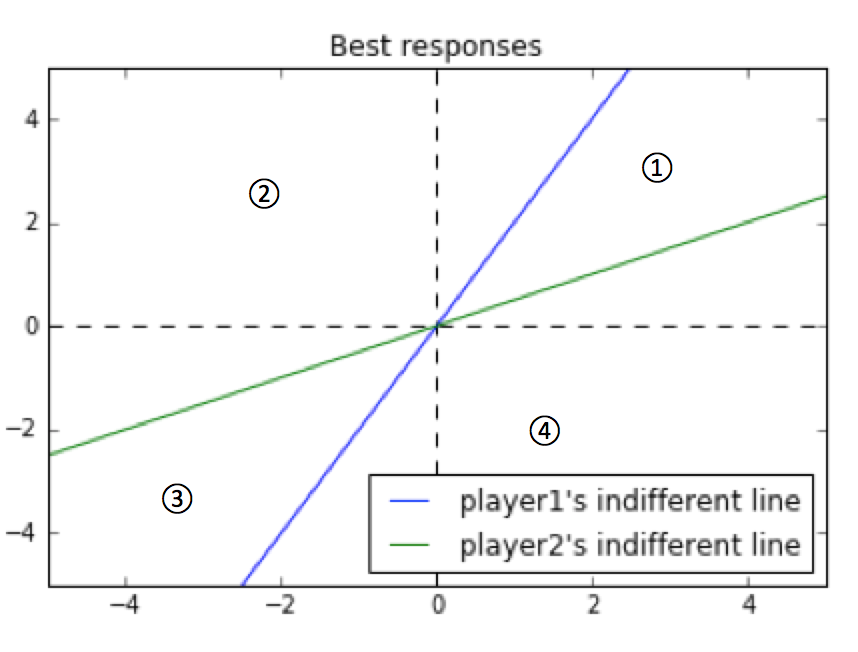
\includegraphics[width=10cm]{BR.png}
    \caption{indifferent curves when $\alpha = -2$}
\end{figure}
$[a, b]$でプレイヤー$1$が電車$a$を、プレイヤー$2$が電車$b$を選ぶことを表現する。これを用いて、相手のタイプが完全にわかっている場合に合理的な行動の結果とられる戦略の組は以下のようであることがわかる。
\begin{align*}
	\begin{cases}
		&[2, 2]\ \text{if}\ (d_1, d_2) \in \text{area 1}\\[8pt]
		&[1, 2]\ \text{if}\ (d_1, d_2) \in \text{area 2}\\[8pt]
		&[1, 1]\ \text{if}\ (d_1, d_2) \in \text{area 3}\\[8pt]
		&[2, 1]\ \text{if}\ (d_1, d_2) \in \text{area 4}\\[8pt]
	\end{cases}
\end{align*}

今簡単のために$d_i \sim N(0,1)\ \forall\ i$とする(global gameのように自分の情報から相手の分布をベイズ推論する方が面白いかも)。プレイヤー$i$は$d_i$のみを観測しているので$d_2$の情報も必要な、上の領域に従った行動の決定はできない。しかしここで$d_i \sim N(0,1)\ \forall\ i$を知っているとすると、自身のタイプである$d_i$に従って、各電車についての最適な選択確率は、すべてのプレイヤー$i$について、
\begin{align*}
	\begin{cases}
	&Pr(\text{i chooses 1}) = 1 - \Phi((1 - \frac{2}{\alpha})d_i)\\[8pt]
	&Pr(\text{i chooses 2}) = \Phi((1 - \frac{2}{\alpha})d_i)
	\end{cases}
\end{align*}
である。ただし、$\Phi(\cdot)$は標準正規分布の累積密度関数である。




\end{document}
























